
\section{Descrizione Architettura}
\subsection{Visione ad alto livello}
\begin{frame}
  \frametitle{Diagramma dei package}
  \begin{center}
    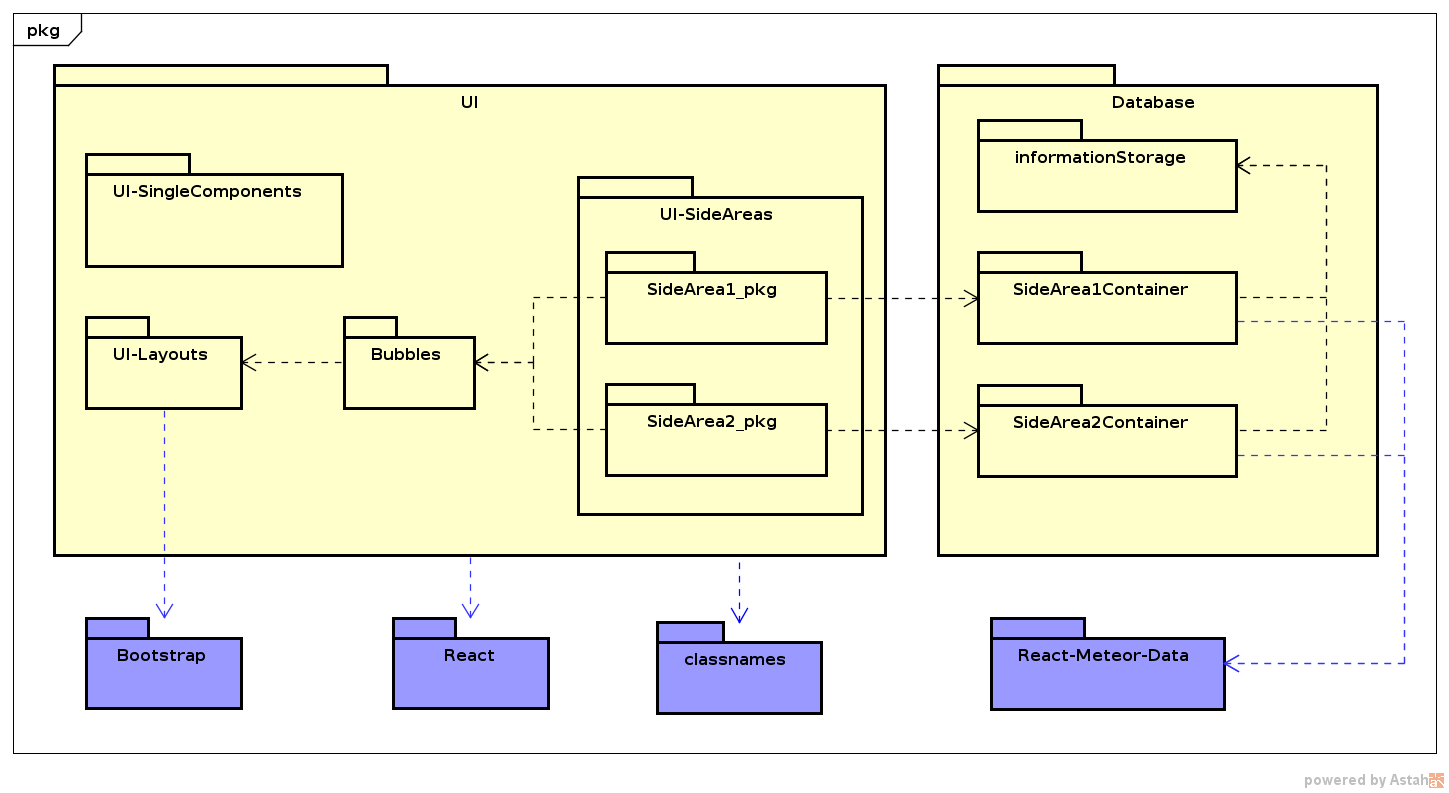
\includegraphics[scale=0.30]{img/General.png}
  \end{center}
\end{frame}


\begin{frame}
  \frametitle{Flusso dei dati }
  \begin{center}
    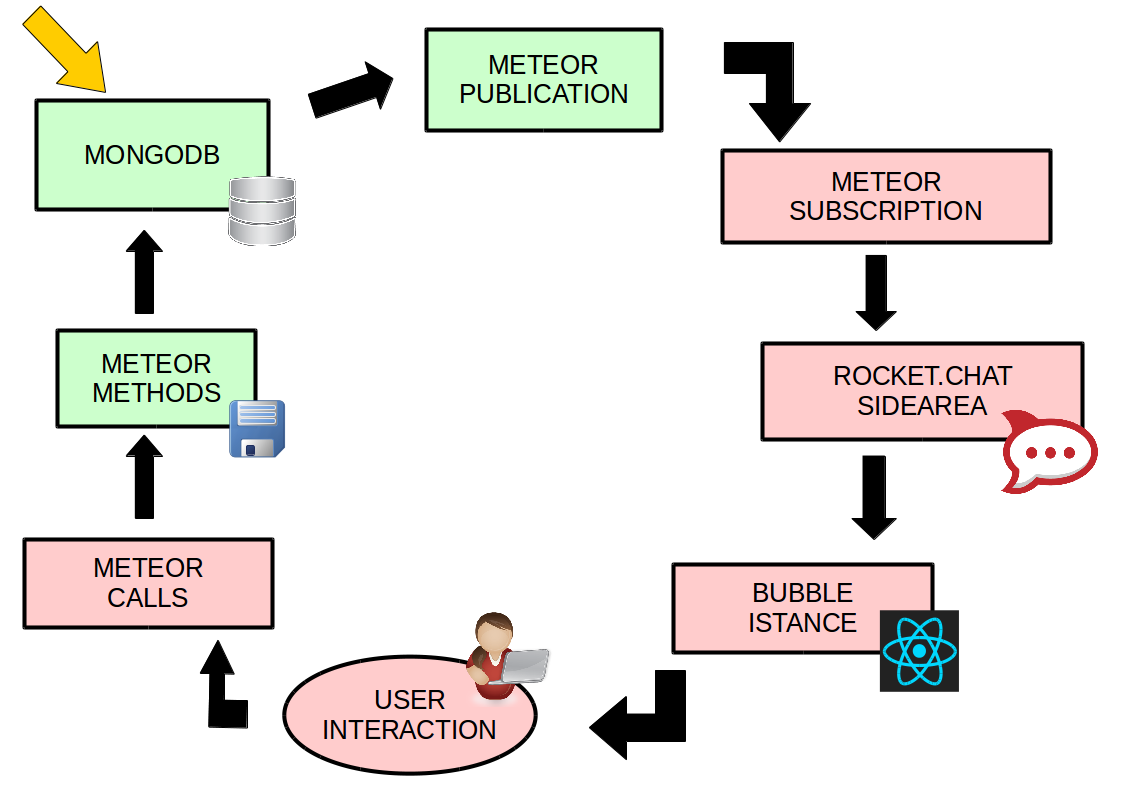
\includegraphics[scale=0.30]{img/2flussodati.png}
  \end{center}
\end{frame}


\subsection{Visione di dettaglio}

\begin{frame}
  \frametitle{Configurazione Database }
  \begin{center}
    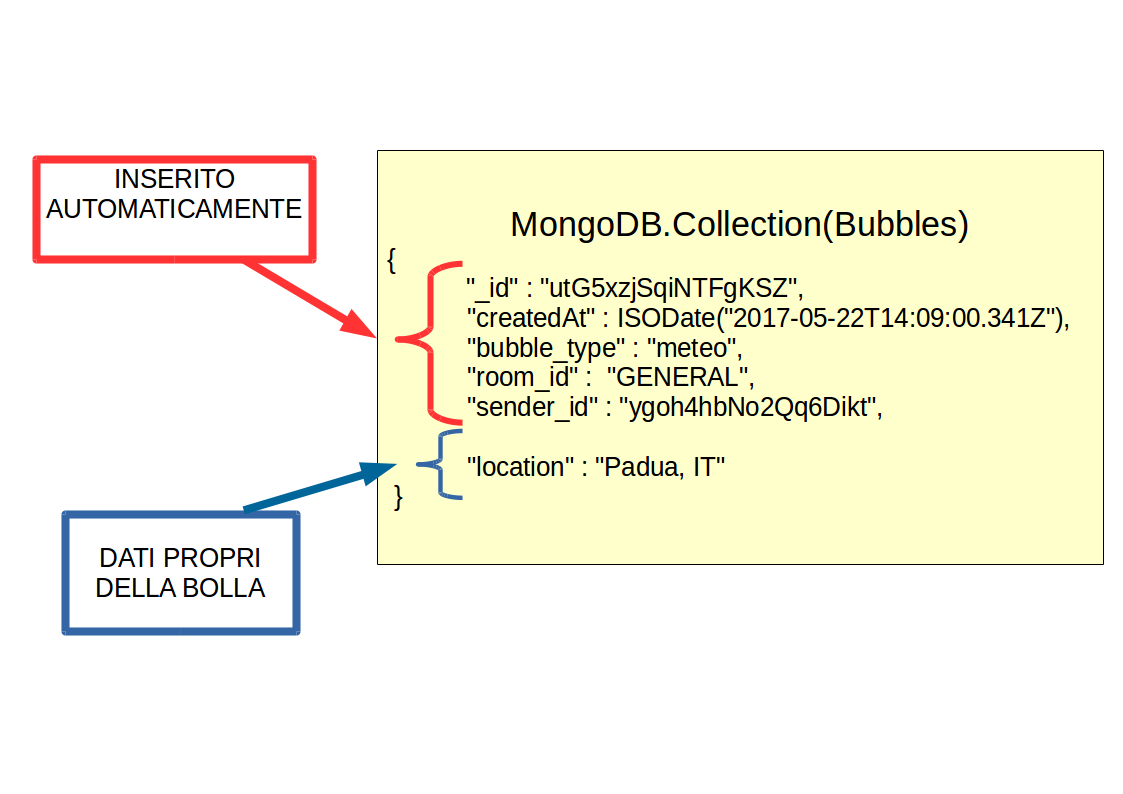
\includegraphics[scale=0.28]{img/1mongo.png}
  \end{center}
\end{frame}


\begin{frame}
  \frametitle{Pubblication \& subscription }
  \begin{center}
    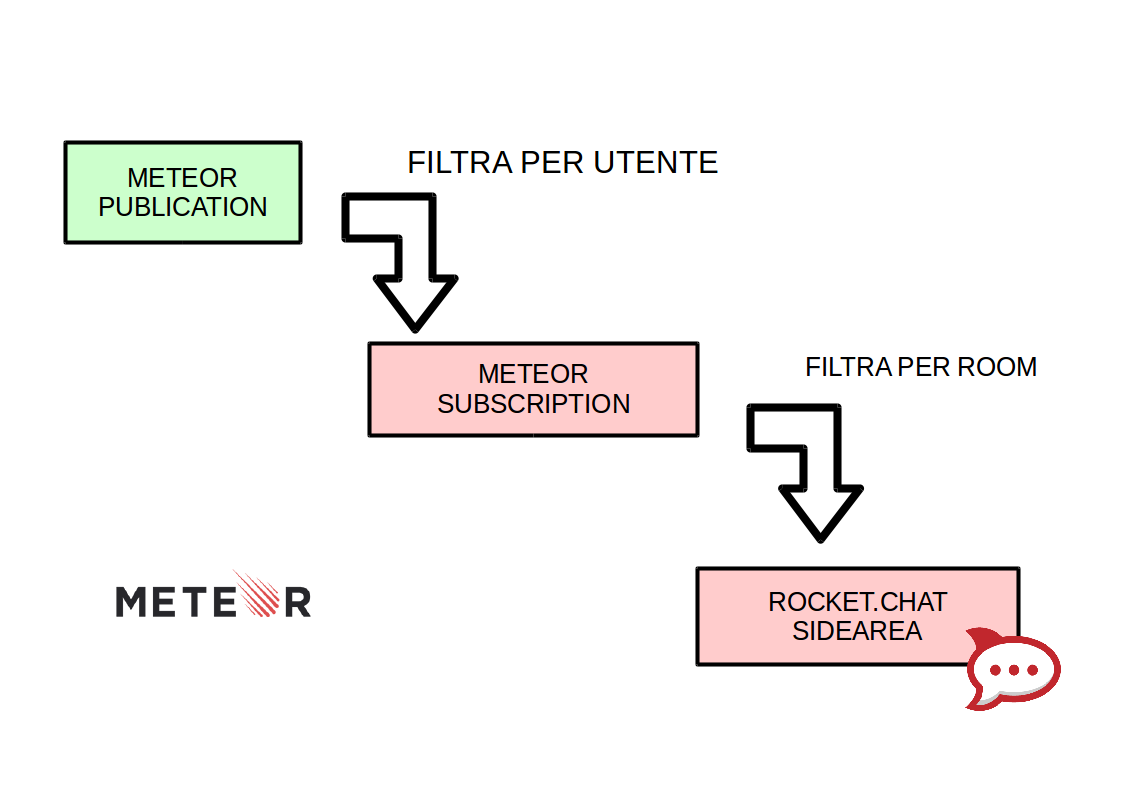
\includegraphics[scale=0.28]{img/3publication.png}
  \end{center}
\end{frame}


\begin{frame}
  \frametitle{Creazione delle bolle }
  \begin{center}
    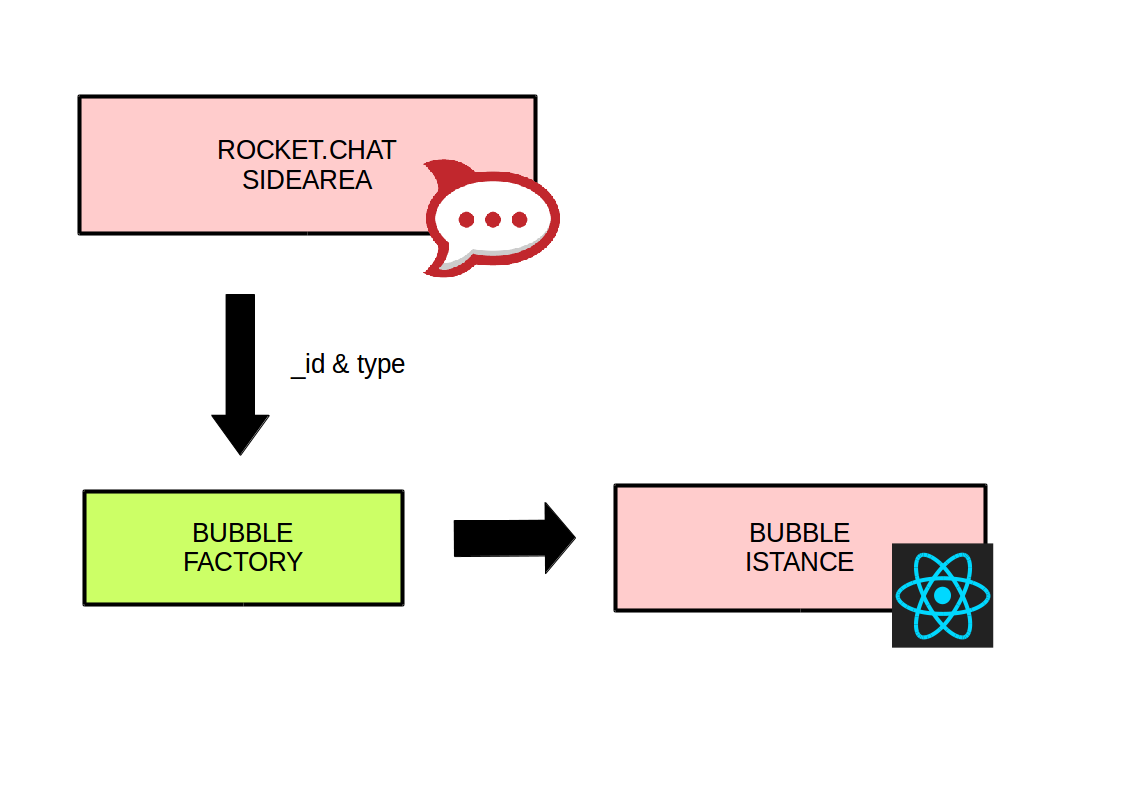
\includegraphics[scale=0.28]{img/4bubbles.png}
  \end{center}
\end{frame}

\begin{frame}
  \frametitle{Diagramma classi per le componenti grafiche }
  \begin{center}
    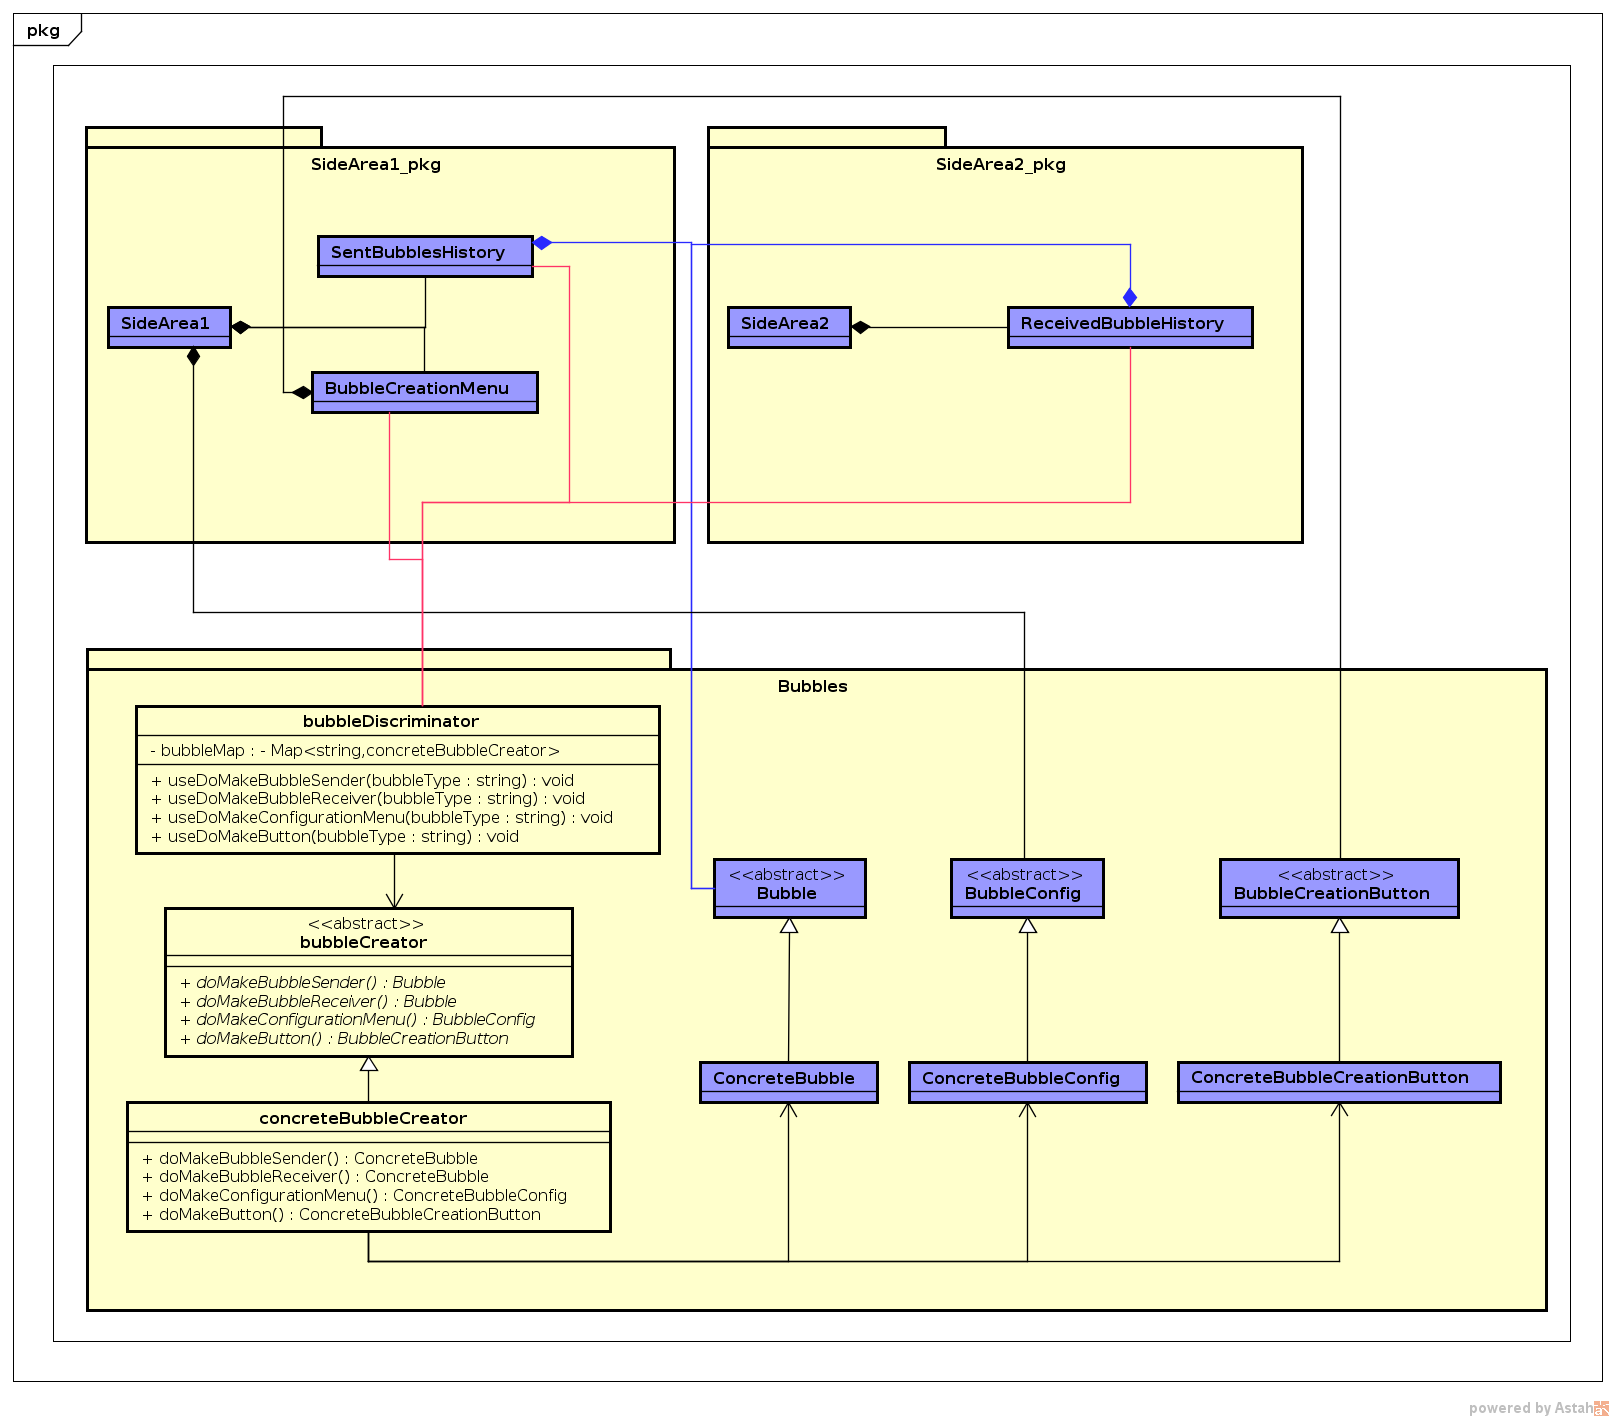
\includegraphics[scale=0.20]{img/Bubbles.png}
  \end{center}
\end{frame}


\begin{frame}
  \frametitle{Meteor.call \& Meteor.methods }
  \begin{center}
    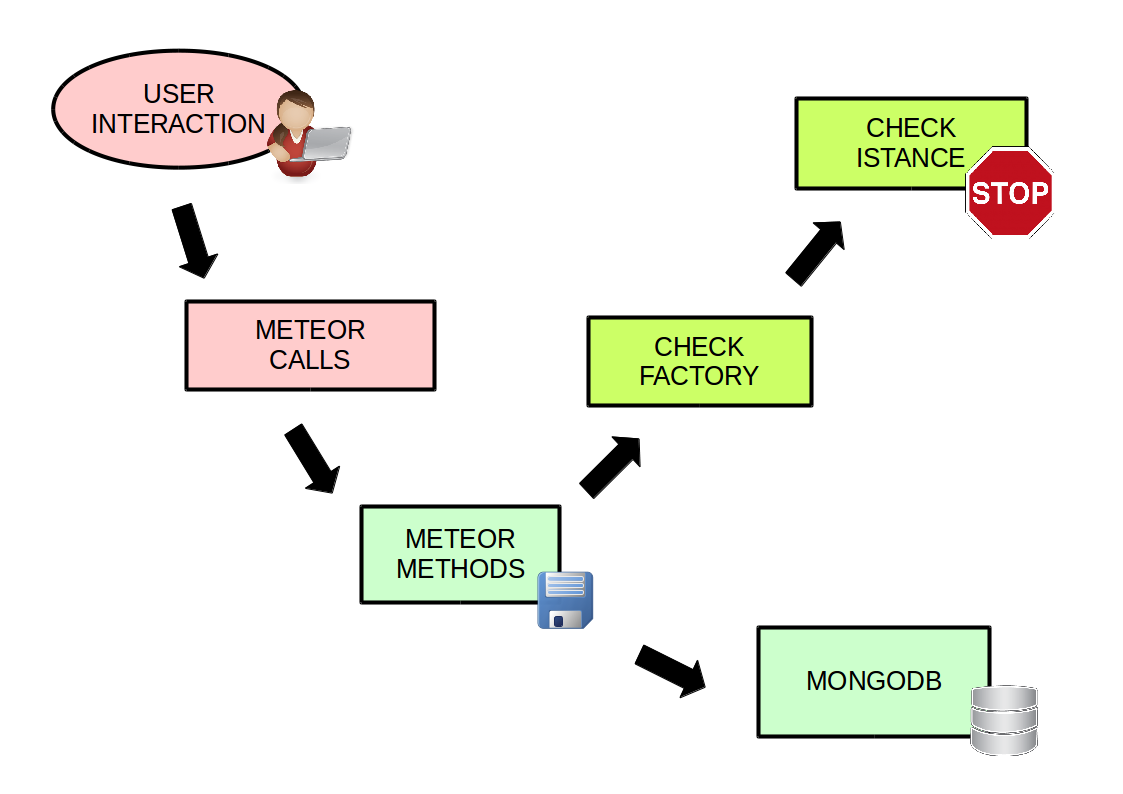
\includegraphics[scale=0.28]{img/5methods.png}
  \end{center}
\end{frame}
